\scanpage{105}

\margin{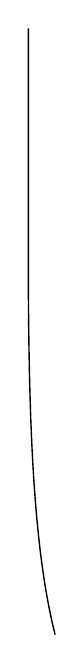
\begin{tikzpicture}\draw[line width=0.5pt] (0,7.7)--(0,4.4).. controls (0.01,2.7) and (0.06,1.1) .. (0.34,0);\end{tikzpicture}}
\textcircled{4} Par l'accouplement \deleted{\unsure{de}}

\[
\langle u,v\rangle=\operatorname{Tr}vu\tag*{\textcircled{26}}
\]

le dual de $L_N(E,F)$ s'identifie à $L^{N^\circ}(F,E)$. Si $E$ et $F$ sont de dimension infinies, \deleted{\unsure{les espaces suivants|les deux conditions} $L_N(E,F)$} \inserted{alors} conditions suivantes sont équivalentes\,: a) $L_N(E,F)$ est réflexif \deleted{$L_N(E,F)=L^N(E,F)$ et $L_{N^\circ}(F,E)=L^{N^\circ}(\unsure{F|F,E})$} b) $L^N(E,F)$ est réflexif c) $\ell^{\deleted{\unsure{\ell|N}}}_{N}$ est réflexif \deleted{\unsure{f),}} d) $\ell_{N'}$ est réflexif. \deleted{\unsure{c'est et seulement si}, \unsure{$\ell$} \unsure{équiv$^{\mathrm{tes}}$ de ces propositions à}\,: d) $\ell^N$ est réflexif. -- e) $\ell_{N^\circ}$ est réflexif et \unsure{enfin} f) $\ell^{N^\circ}$ est réflexif)} \deleted{\unsure{alors}} d) $L_N(E,F)=L^N(E,F)$ et $\begin{aligned}&L_{N^\circ}(F,E)=L^{N^\circ}(F,E)\\[-0.5ex]&\quad\text{\deleted{\unsure{et}}}\end{aligned}$

\textcircled{5} \deleted{\unsure{Remarquons|Remarque}} Soit $u\in L_0(E,F)$, \deleted{si $u\in L^N(E,\unsure{F|E})$\unsure{,} \unsure{alors} \unsure{Alors} $(\lambda_i(u))\in\ell^N$,} \inserted{Alors}

\[
N((\lambda_i(u)))\leq\deleted{N(\unsure{(\rho_i(u))|(\rho_i u)})}N(u)\tag*{(27)}
\]

Si $u\in L^N(E,F)$, \deleted{alors (resp$^t$ $L_N(E,E)$)} alors, $(\lambda_i(u))\in\deleted{\unsure{\ell_N|L^N\unsure{,}|\ell^N}}\ell^N$ \deleted{(resp$^t$ $\ell_N$)}

Tout est démontré, sauf 4. \deleted{\unsure{et}} et 5. Pour 4, on note\,: si $E$ et $F$ sont de dimension infinie, alors $\ell^N$ \inserted{(resp$^t$ $\ell_N$)} est isométrique à un sous-espace vectoriel normé de $L^N(E,F)$ (resp$^t$ $L_N(E,F)$. (\textcolor{red}{\uline{\textcolor{black}{prendre}}} $(e_i)$, $(f_i)$ systèmes orthonormaux infinis, et $(\lambda_i)\to\sum\lambda_i\bar e_i\otimes f_i$ de $\ell^N$ dans $L^N(E,F)$). \deleted{Donc}

Si $L^N_{\deleted{\unsure{0|N}}}(E,F)$ est réflexif, $L_N(E,F)$ est réflexif, et alors aussi $\ell_N$ est réflexif, \deleted{\unsure{donc}}\inserted{\unsure{Celà|ce q.} implique} (voir --) $\ell_N=\ell^N$, $\ell_{N^\circ}=\ell^{N^\circ}$, donc $L^N(E,F)=L_N(E,F)$ (car on \deleted{\unsure{peut supposer}}\inserted{aura} exigé $N\unsure{\not\simeq|\neq}N_\infty$), donc $L^N(E,F)$ sera réflexif, d'où l'équivalence a), b), c).

\margin{
\begin{tikzpicture}\draw[red,line width=0.65pt] (0,2.35).. controls (0.09,1.55) and (0.10,0.75) .. (0.19,0.48);\draw[red,line width=0.45pt] (0.04,1.34).. controls (0.02,0.79) and (0.07,0.31) .. (0.12,0);\end{tikzpicture}}
Et le fait que cela implique d) (d'abord la première assertion, pour la seconde on $\ell_{N^\circ}$ sera aussi réflexif). Enfin d implique \deleted{$\ell_N=\ell^N$ et $\ell_{N^\circ}=\ell^{N^\circ}$ (voir \unsure{théorème précédent|th. précédent}) donc $\ell_N$ réflexif (\unsure{toujours|voir --})} \inserted{que le dual de $L_N(E,F)$ est $L_{N^\circ}(F,E)$,} dont le dual est $L_N(E,F)$, donc $L_N(E,R)$ est réflexif.

\textcircled{5} (27) Est le corollaire 5 du 1. th. de convexité \deleted{\unsure{Résulte aussitôt du|résulte immédiatement}}
\margin{106}
